\documentclass[ignorenonframetext,8pt,aspectratio=169]{beamer}

\usepackage{umut}
\usepackage{umuttr}
\usepackage{usynsem}
\usepackage[utf8]{inputenc}
\usepackage{uling}
\usepackage{natbib,unatbib}
\usepackage{linguex}
         \renewcommand{\refdash}{}
\usepackage{ubeamer}
\usepackage{verbatim}
\usepackage{adjustbox}
\usepackage{fancyvrb}

\usepackage{ulem}

\usepackage{tikz-qtree}
\usetikzlibrary{er,positioning}

\title{Minimal Search}
\author{\  \\  {\it Based on Koeneman \& Zeiljstra (2017)} \\ \vspace{20pt} Umut \"Ozge\\  }

\date{COGS 532: Theoretical Linguistics\\ METU, Informatics}

\begin{document}

\begin{frame}\frametitle{}
\thispagestyle{empty}
\maketitle
\end{frame}

\begin{frame}[t,plain]{Subject movement to FinP}

\ex. Mary sleeps. 

\vspace{20pt}
\hspace{80pt}
\begin{tikzpicture}
\tikzset{level distance=20pt, sibling distance=25pt}
\tikzset{every tree node/.style={align=center,anchor=north}}

\Tree[.{FinP} [.{DP} Mary\\{\begin{avm} \[cat  & n \\ det & + \\ $\phi$  & 3, sg\ \\ {finite$^{(u)}$} & {+} \]  \end{avm}} ] [.{Fin'} [.{Fin} -s\\{\begin{avm} \[cat  & fin \\ finite  & + \\ {$\phi^{(u)}$}  & {3, sg} \] \end{avm}}  ] [.{VP} [.{<DP>} Mary\\{\begin{avm} \[cat  & n \\ det & + \\ $\phi$  & 3, sg\ \\ {finite$^{(u)}$} & {+} \]  \end{avm}} ] [.{V} sleep\\{\begin{avm} \[cat  & v \\ \] \end{avm}} ] ] ] ] 
\end{tikzpicture}
\end{frame}

\begin{frame}[t,plain]{Why move the subject?}

\ex.
\a. *Often has Mary kissed Eve.
\b. *In the garden kisses Mary Eve. 

\end{frame}

\begin{frame}[t,plain]{Why move the subject?}
\ex. *Her has she kissed <her>.

\vspace{20pt}
\hspace{30pt}
\begin{tikzpicture}
\tikzset{level distance=20pt, sibling distance=25pt}
\tikzset{every tree node/.style={align=center,anchor=north}}

\Tree[.{FinP} [.{DP} Her\\{\begin{avm} \[$\phi$  & 3,sg \\ cat$^{(u)}$  & v\] \end{avm}} ] [.{Fin'} [.{Fin} has\\{\begin{avm} \[cat  & fin \\ finite  & + \\ $\phi^{(u)}$  & 3,sg\] \end{avm}} ] [.{VP} [.{DP} she\\{\begin{avm} \[cat  & n \\ det  & + \\ $\phi$  & 3,sg \\ finite$^{(u)}$  & +\] \end{avm}} ] [.{V'} [.{V} kissed\\{\begin{avm} \[cat  & v \]\end{avm}} ] [.{<DP>} her\\{\begin{avm} \[$\phi$  & 3,sg \\ cat$^{(u)}$  & v\] \end{avm}} ] ] ] ] ] 



\end{tikzpicture}
\end{frame}

\begin{frame}[t,plain]{Minimal Search}

\ex. When you need to remerge a constituent with some interpretable feature \setavm{\[F\]} to check off some uninterpretable feature \setavm{\[F$^{(u)}$\]} on some other constituent, search for the closest constituent with \setavm{F} that is c-commanded by the element with \setavm{\[F$^{(u)}$\]}.

\end{frame}

\begin{frame}[t,plain]{An intricacy of Minimal Search}

\ex. *Them have Mary loved <them>.

\end{frame}

\begin{frame}[t,plain]{The passive}


\vspace{20pt}
\hspace{60pt}
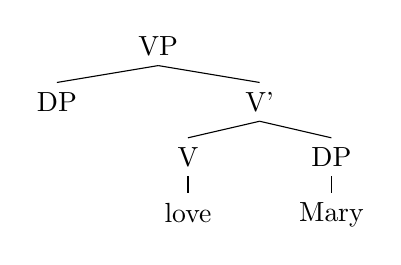
\begin{tikzpicture}
\tikzset{level distance=20pt, sibling distance=25pt}
\tikzset{every tree node/.style={align=center,anchor=north}}

\Tree[.{VP} [.{DP} ] [.{V'} [.{V} love ] [.{DP} Mary ] ] ] 


\end{tikzpicture}
\hspace{50pt}
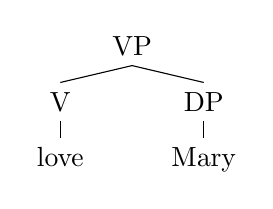
\begin{tikzpicture}
\tikzset{level distance=20pt, sibling distance=25pt}
\tikzset{every tree node/.style={align=center,anchor=north}}

\Tree[.{VP} [.{V} love ] [.{DP} Mary ] ] 

\end{tikzpicture}

\end{frame}

\end{document}
